\documentclass[12pt,a4paper]{article}
\usepackage{amsmath}
\usepackage{mathtext}
\usepackage{icomma}
\usepackage{amsfonts}
\usepackage{amssymb}
\usepackage[utf8]{inputenc}
\usepackage[T1,T2A]{fontenc}
\usepackage[english, russian]{babel}
\usepackage{graphicx}
\usepackage[left=2cm,right=2cm,top=2cm,bottom=2cm]{geometry}
\usepackage{calc}
\usepackage{wrapfig}
\usepackage{setspace}
\usepackage{indentfirst}
\usepackage{subfigure}
\usepackage[table,xcdraw]{xcolor}
\usepackage{float}

\title{Отчет о выполнении лабораторной работы 3.2.2(4.8)\\
Резонанс напряжений}

\author{Исламов Сардор, группа Б02-111}
\date{22 октября 2022 г.}
\begin{document}
\maketitle
\subparagraph*{Аннотация.} 
В данной работе исследован резонанс напряжений в последовательном колебательном контуре с изменяемой ёмкостью, также исследован закон Ома.

\subsection*{Теоретическое введение}
% В колебательный контур рассматриваемых установок добавлен постоянный резистор $R$ (см. рис. 1), снижающий его добротность. 
% Это сделано для упрощения процедур получения и обра­ ботки резонансных кривых. Таким образом, суммарное активное сопро­ тивление контура принимается равным
% \[R_\Sigma = R + R_L +R_S,\]
% где $R_S = \dfrac{\tan \delta }{\omega C}$.
% Добротность контуров тем не менее остаётся достаточно высокой, чтобы можно было пользоваться формулами 
% \[Q \approx \dfrac{\omega_0}{2\gamma} = \dfrac{\pi}{\gamma T_0} = \dfrac{\tau \omega_0}{2} = \dfrac{1}{R}\sqrt{\dfrac{L}{C}} = \dfrac{\rho}{R} \gg 1,\]
% в которых надо учитывать суммарное активное сопротивление контура:
% \begin{equation}
%     Q = {\rho \over R_\Sigma} = {\omega_0L\over R_\Sigma} = {1 \over \omega_0 CR_\Sigma} \gg 1.
% \end{equation}

% Для импедансов ёмкости $ZC$, индуктивности $ZL$ и последовательного контура $Z = Z_L + R + Z_C$ с учётом (1) получаем выражения
% \begin{equation}
%     Z_C = R_S - {i\over \omega C}, \quad Z_L = R_L + i\omega L, \quad Z = R_\Sigma + i\left( \omega L - {1\over \omega C}\right)
% \end{equation}

% Комплексные амплитуды тока в контуре $I = E / Z$ и напряжений на сопротивлении $U_R = RI$, ёмкости $U_C = Z_CL$ и индуктивности $U_L = Z_LI$ при нулевой начальной фазе $\varphi_0$ напряжения на контуре $\varepsilon = \varepsilon_0e^{i\varphi_0}$ удобно записать в виде
% \begin{equation}
%     I = {U_R \over R} = {\varepsilon_0 \over R_\Sigma} {1 \over 1 + iQ(\omega/\omega_0 - \omega_0/\omega)}
% \end{equation}

% \begin{equation}
%     U_C = -iQ\varepsilon_0 {\omega_0 \over \omega} {1 + i \tan \delta \over 1 + iQ(\omega/\omega_0 - \omega_0/\omega)}
% \end{equation}

% \begin{equation}
%     U_L = iQ\varepsilon_0 {\omega \over \omega_0} {1 - i R_L/\rho \over 1 + iQ(\omega/\omega_0 - \omega_0/\omega)}
% \end{equation}

% Наибольший практический интерес представляет случай, когда от­ клонение $\Delta \omega = \omega - \omega_0$ частоты внешней ЭДС от собственной частоты контура $\omega_0$ удовлетворяет сильному неравенству $|\Delta \omega| \ll \omega_0$. 
% При этом в первом порядке малости по относительной расстройке часто­ты $\Delta \omega / \omega_0$
% \[{\omega \over \omega_0} - {\omega_0 \over \omega} = {2 \Delta \omega \over \omega_0}\],
% что позволяет упростить выражения (3) - (5) и представить веществен­ные части комплексных амплитуд и соответствующих им фаз в виде
% \begin{equation}
% 	I = \frac{\varepsilon_0}{R_\Sigma} \frac{\cos(\omega t - \psi_I)}{\sqrt{1+(\tau \Delta \omega )^2}}, \quad \psi_I = \arctan(\tau \Delta \omega)
% \end{equation}
% \begin{equation}
% 	U_C = \varepsilon_0 Q \frac{\omega_0}{\omega} \frac{\cos(\omega t - \psi_C)}{\sqrt{1+(\tau \Delta \omega )^2}}, \quad \psi_C = \psi_I + {\pi \over 2} - \delta
% \end{equation}
% \begin{equation}
% 	U_L = \varepsilon_0 Q \frac{\omega_0}{\omega} \frac{\cos(\omega t - \psi_L)}{\sqrt{1+(\tau \Delta \omega )^2}},\quad \psi_L = \psi_I - {\pi \over 2} + {R_L \over \rho}.
% \end{equation}
% Здесь $\tau$ — время затухания.

% При резонансе, когда для высокодобротного контура можно поло­ жить $\Delta \omega = 0$, выражения для модулей комплексных амплитуд тока и напряжения на ёмкости и их фаз принимают вид
% \begin{equation}
%     I(\omega_0) = {\varepsilon \over R_\Sigma}, \quad \psi_I(\omega_0) = 0,
% \end{equation}

% \begin{equation}
%     U_C(\omega_0) = Q\varepsilon_0, \quad \psi_C(\omega_0) = {\pi \over 2} - \delta,
% \end{equation}

% \begin{equation}
%     U_L(\omega_0) = Q\varepsilon_0, \quad \psi_L(\omega_0) = -{\pi \over 2} + {R_L \over \rho}.
% \end{equation}

Рассмотрим электрическую цепь, состоящую из резистора $ R $ и катушки индуктивности $ L $ с импедансом $ Z_L = r_L + i \Omega L $, последовательно подключённых к внешнему источнику, ЭДС которого меняется по синусоидальному закону с частотой (рис. 1).

Обозначим через $ U_R $ напряжение на резисторе, через $ U_L $ -- напряжение на катушке и через $ U_{R+L} $ — суммарное напряжение на катушке и на резисторе. Для этих напряжений справедливы комплексные соотношения:
\begin{equation}\label{eq:1}
{\widehat U_R} = \widehat IR, \quad {\widehat U_L} = \widehat I\left( {{r_L} + i\Omega L} \right), \quad {\widehat U_{R + L}} = \widehat I\left( {R + {r_L} + i\Omega L} \right).
\end{equation}
Напомним, что здесь $ r_L $ -- активное сопротивление катушки, которое характеризует суммарные потери энергии в катушке, в том числе потери в её ферромагнитном сердечнике.

Переходя к модулям и фазам токов и напряжений, найдём из (\ref{eq:1}):
\begin{equation}\label{eq:2}
{U_R} = I \cdot R, \quad \tg{\psi _1} = 0;
\end{equation}
\begin{equation}\label{eq:3}
{U_L} = I \cdot \sqrt {r_L^2 + {{\left( {\Omega L} \right)}^2}}, \quad \tg{\psi _2} = \frac{{\Omega L}}{{{r_L}}};
\end{equation}
\begin{equation}\label{eq:4}
{U_{R + L}} = I\sqrt {{{\left( {R + {r_L}} \right)}^2} + {{\left( {\Omega L} \right)}^2}}, \quad \tg{\psi _3} = \frac{{\Omega L}}{{R + {r_L}}}.
\end{equation}
В этих формулах $ U $ и $ I $ обозначают \textit{эффективные} значения напряжений и токов (показания приборов), как принято в электротехнике.

Измеряя с помощью трёх вольтметров значения $ U_R $, $ U_L $ и $ U_{R+L} $ и зная сопротивление резистора $ R $, нетрудно вычислить, пользуясь формулами (\ref{eq:2}), (\ref{eq:3}) и (\ref{eq:4}), силу тока в цепи, активное сопротивление катушки $ r_L $, её индуктивность $ L $, мощность $ P_L $, выделяемую на катушке, и сдвиг фаз между током и напряжением на катушке.

Рассчитаем мощность переменного тока, выделяемую в катушке. Мгновенное значение мощности равно
\begin{equation*}
P = U\left( t \right) \cdot I\left( t \right).
\end{equation*}
Средняя мощность за период $ T $ определяется формулой
\begin{equation*}
\overline P  = \frac{1}{T}\int\limits_0^T {U\left( t \right) \cdot I\left( t \right)dt}.
\end{equation*}
Полагая $ \displaystyle I\left( t \right) = I\sqrt 2 \cos \Omega t $, $ U\left( t \right) = U\sqrt 2 \cos \left( {\Omega t + \psi } \right) $, получим после интегрирования:
\begin{equation}\label{eq:5}
{P_L} = {U_L} \cdot I\cos \psi  = {I^2} \cdot {r_L}.
\end{equation}
Средняя мощность, выделяющаяся в катушке самоиндукции, определяется, таким образом, действительной частью её импеданса.

Активное сопротивление катушки $ r_L $ можно определить, если включить её в последовательный колебательный контур с известными параметрами -- сопротивлением $ R $ и ёмкостью $ C $ (рис. ). В контуре, настроенном в резонанс на частоту $ \Omega $ внешнего источника (собственная частота контура и внешняя совпадают: $ \omega_0 = \Omega $, реактивные сопротивления индуктивности и ёмкости одинаковы:
\begin{equation}\label{eq:6}
{\omega _0}L = \frac{1}{{{\omega _0}C}}.
\end{equation}
Определив каким-либо экспериментальным способом добротность $ Q $ этого контура, можно рассчитать полное сопротивление контура $ R_{\Sigma} $ в резонансе, поскольку
\begin{equation}\label{eq:7}
Q = \frac{{{\omega _0}L}}{{{R_\Sigma }}} = \frac{1}{{{\omega _0}C{R_\Sigma }}}.
\end{equation}
Резонансное сопротивление контура $ R_{\Sigma} $, включает в себя известное со противление резистора $ R $ и активное сопротивление катушки $ r_L $:
\begin{equation}\label{eq:8}
{R_\Sigma } = R + {r_L}.
\end{equation}

\subsection*{Экспериментальная установка}
В данной работе изучаются резонансные явления в последователь­ном колебательном контуре (резонанс напряжений). 
Схема эксперимен­тального стенда показана на рис. 1. 
\begin{wrapfigure}{l}{0.5\linewidth}
    \centering
    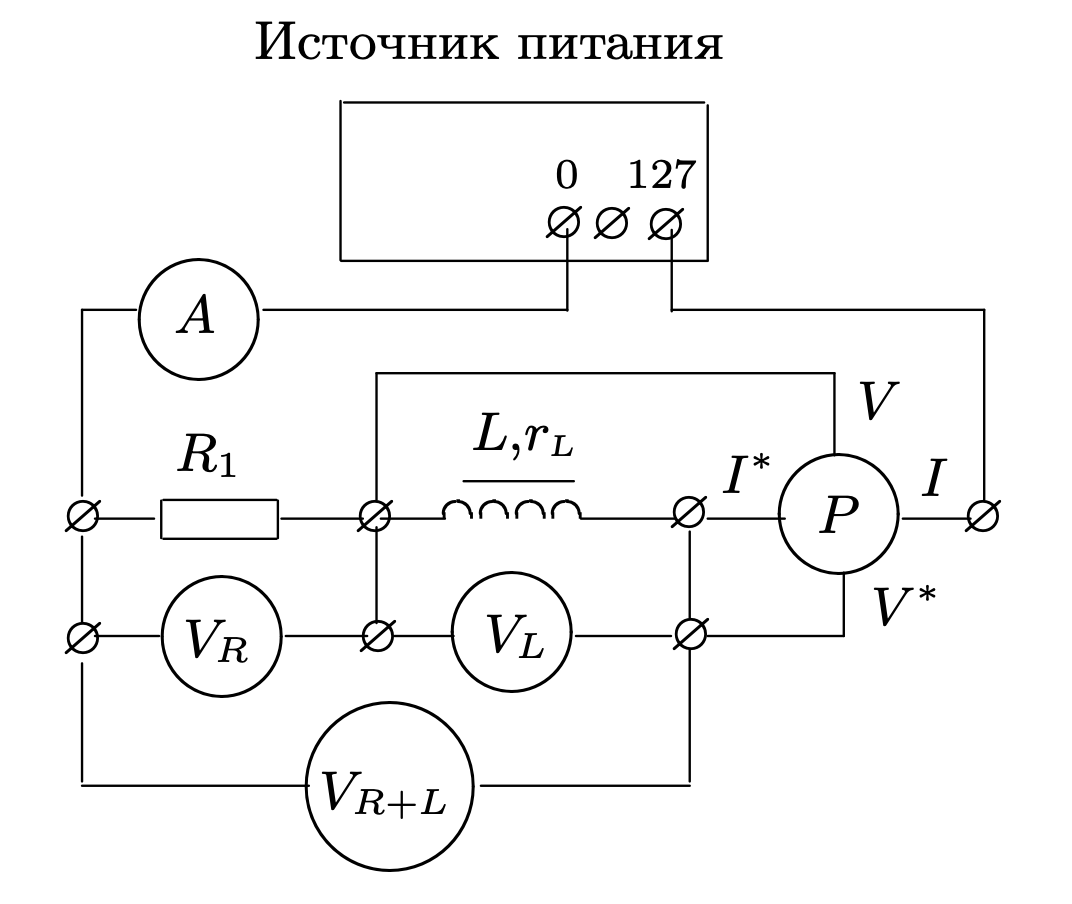
\includegraphics[width=\linewidth]{pics/scheme1.png}
    \caption{Схема установки для изучения закона Ома в цепи переменного тока}
\end{wrapfigure}
% Синусоидальный сигнал от гене­ратора поступает на вход управляемого напряжением источника на­пряжения, собранного на операционном усилителе, питание которого осуществляется встроенным блоком–выпрямителем от сети $\sim$220 В (цепь питания на схеме не показана). 
% Источник напряже­ния (источник с нулевым внутренним сопротивлением) обеспечивает с высокой точностью постоянство амплитуды сигнала $\varepsilon = \varepsilon_0 \cos(\omega t + \varphi_0)$ на меняющейся по величине нагрузке — последовательном колебатель­ ном контуре, изображённом на рис. 1 в виде эквивалентной схемы.

% Источник напряжения, колебательный контур и блок питания за­ключены в отдельный корпус, отмеченный на рисунке штриховой лини­ей. 
% На корпусе имеются коаксиальные разъёмы «Вход», «$U_1$» и «$U_2$», а также переключатель магазина ёмкостей $C_n$ с указателем номера $n = $ 1, 2, ... 7. 
% Величины ёмкостей $C_n$ указаны на установке. 
% Напря­жение $\varepsilon$ на контуре через разъём «$U_1$» попадает одновременно на ка­нал 1 осциллографа и вход 1-го цифрового вольтметра.
% Напряжение на конденсаторе $U_C$ подаётся через разъём «$U_2$» одновременно на канал 2 осциллографа и вход 2-го цифрового вольтметра.
Схема установки для исследования закона Ома в цепи переменного тока представлена на рис. 1. 
Цепь, состоящая из резистора $R_1 \simeq 100$ Ом и катушки $L$ с выдвижным сердечником, подключена к автотрансформатору, выходное напряжение которого можно менять от 0 до 127 В. 
Напряжения на каждом из элементов и суммарное напряжение цепи измеряются тремя вольтметрами: $V_R,\ V_L\ и\ V_{R+L}$. 
Амперметр A измеряет ток в цепи, а ваттметр P — мощность, выделяющуюся на катушке.

Ваттметр электродинамической системы состоит из двух катушек, одна из которых вращается в магнитном поле другой, если через них течёт ток. 
Токовая катушка ваттметра $II^*$ включается последовательно в исследуемую цепь, а катушка напряжений (потенциальная) $VV^*$ — параллельно к элементу, в котором измеряется выделяемая мощность.

Два из четырёх зажимов ваттметра помечены звёздочкой (*). 
Эти зажимы надо соединить вместе. 
Предел измерений устанавливается при помощи переключателей или штепселей, которые вставляются в соответствующие гнёзда: произведение цифр против штепселя токовой катушки $II^*$ и против переключателя катушки напряжений $VV^*$ определяет мощность, соответствующую отклонению стрелки на всю шкалу. 
Отсчёт мощности ведётся по любой из шкал, обозначенных буквой $P$.

\begin{wrapfigure}{l}{0.5\textwidth}
    \centering
    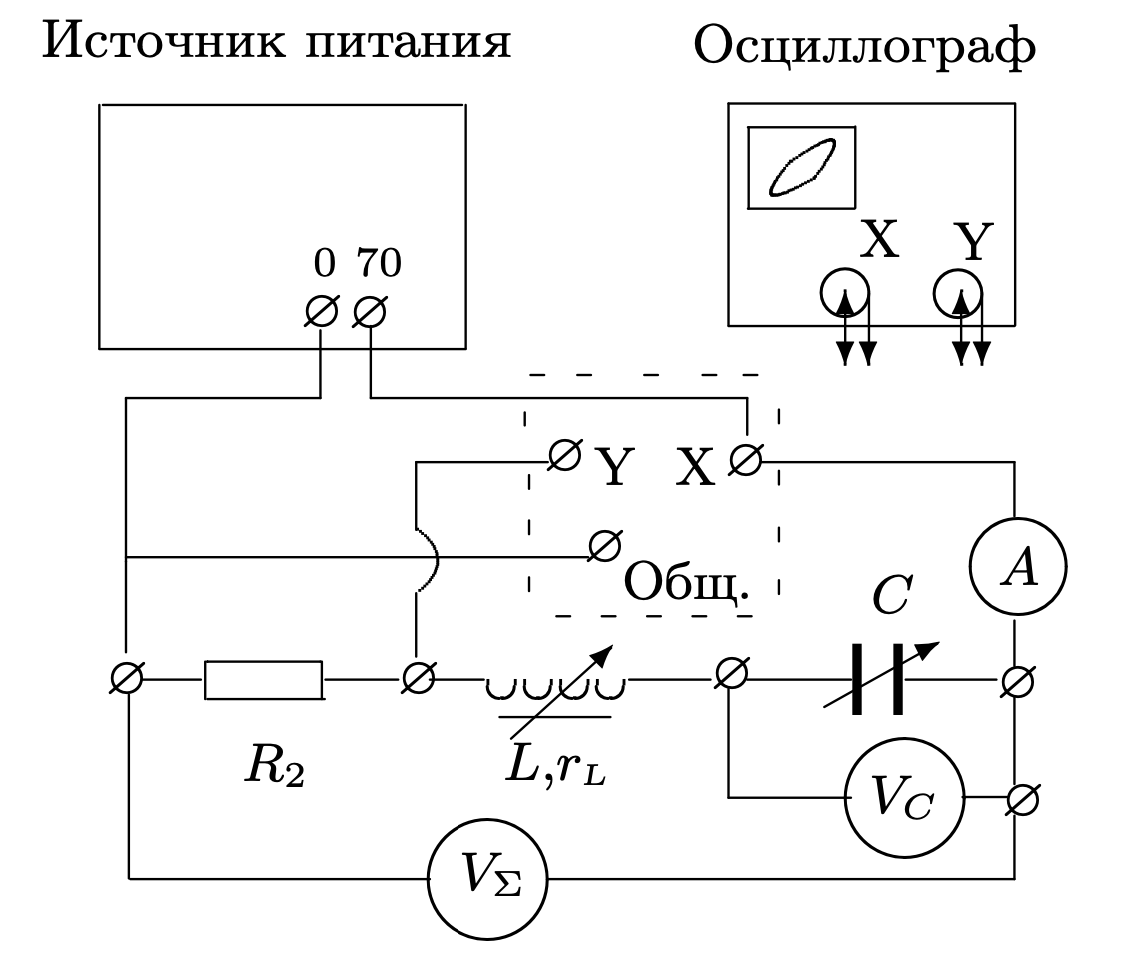
\includegraphics[width=\linewidth]{pics/scheme2.png}
    \caption{Схема установки для наблюдения резонанса напряжений}
\end{wrapfigure}

Схема установки для изучения резонанса напряжений изображена на рис. 2. 
Последовательно соединены резистор $R_2 \simeq 5$ Ом, катушка $L$ и магазин емкостей $C$. 
Амперметр $A$ измеряет ток в цепи, вольтметр $V_C$ — напряжение на ёмкости, вольтметр $V_\Sigma$ — суммарное напряжение на контуре. 
Резонанс можно зафиксировать с помощью осциллографа, если подать на вход $X$ напряжение с контура, а на вход $Y$ — напряжение с резистора $R_2$, пропорциональное току в цепи. 
В общем случае на экране виден эллипс. 
При резонансе эллипс вырождается в прямую линию.
\newline
\newline
\newline
\newline

\subsection*{Результаты измерений и обработка данных}
\subparagraph*{Закон Ома в цепи переменного тока.} 
Установим зависимость параметров цепи от индуктивности катушки. 
Для этого будем малыми шагами изменять положение сердечника и снимать показания с приборов (табл. 1).
Сопротивление реостата $R_1 = 98$ Ом. 
Установленные на приборах пределы измерения, а также их параметры в установленных режимах указаны в табл. 2

\begin{table}[H]
	\centering
	\begin{tabular}{|l|c|c|c|c|c|c|c|c|c|}
	\hline
	$x$, мм      & 5    & 7     & 9   & 11   & 13    & 15   & 17   & 19    & 21  \\ \hline
	$I$, дел     & 32   & 35    & 37  & 38   & 39.5  & 40   & 40.5 & 41    & 41  \\ \hline
	$U_R$, дел  & 67   & 72.5  & 77  & 80   & 82    & 83.5 & 84.5 & 85.5  & 86  \\ \hline
	$U_{RL}$, дел & 117  & 115.5 & 114 & 113  & 112.5 & 112  & 111  & 110.5 & 110 \\ \hline
	$U_L$, дел  & 80   & 72.5  & 65  & 60.5 & 56.5  & 52.5 & 50   & 47.5  & 45  \\ \hline
	$P_L$, дел  & 47.5 & 43    & 40  & 38   & 36    & 34   & 33   & 32    & 31  \\ \hline
	\end{tabular}
	\caption{Зависимость величин в цепи от индуктивности}
\end{table}

\begin{table}[H]
	\centering
	\begin{tabular}{|l|c|c|c|c|c|c|c|c|c|}
	\hline
	 & Предел измерений & Сопротивление & Индуктивность & Класс точности\\ \hline
	$I$ & 5А / 100 дел & 0.005 Ом & 0.0023 мГн & 0.5\\ \hline
	$U_R$ &75В / 150 дел & 1667 Ом & $-$ & 0.5 \\ \hline
	$U_{RL}$ & 150В / 150 дел & 2.5 кОм & $-$ & 0.5 \\ \hline
	$U_L$ & 150В / 150 дел & 2.5 кОм & $-$ & 0.5 \\ \hline
	$P_L$ & 250Вт / 100 дел & $-$ & $-$ & 0.5\\ \hline
	\end{tabular}
	\caption{Параметры приборов}
\end{table}

Теперь по формулам (5) и (3) вычислим $r_L$ и $L$ (табл. 3) и изобразим на графиках (рис. 3) их зависимости от положения сердечника.

\begin{table}[H]
	\centering
	\begin{tabular}{|l|c|c|c|c|c|c|c|c|c|}
	\hline
	$x$, мм      & 5    & 7     & 9   & 11   & 13    & 15   & 17   & 19    & 21  \\ \hline
	$r_L,$ 10  Ом           & 4.64 & 3.51 & 2.92 & 2.63 & 2.31 & 2.12 & 2.01 & 1.9  & 1.84 \\ \hline
	$\sigma_{r_L}$, 10 Ом   & 0.15 & 0.11 & 0.09 & 0.08 & 0.07 & 0.06 & 0.06 & 0.06 & 0.05 \\ \hline
	$L, 10^{-2} Гн$         & 5.94 & 7.0  & 6.21 & 5.71 & 5.38 & 4.91 & 4.56 & 4.2  & 3.79 \\ \hline
	$\sigma_L, 10^{-2} Гн$ & 0.25 & 0.13 & 0.1  & 0.09 & 0.08 & 0.07 & 0.07 & 0.07 & 0.07 \\ \hline
	\end{tabular}
	\caption{Зависимость $r_L$ и $L$ от $x$}
\end{table}

\begin{figure}[H]
	\centering
	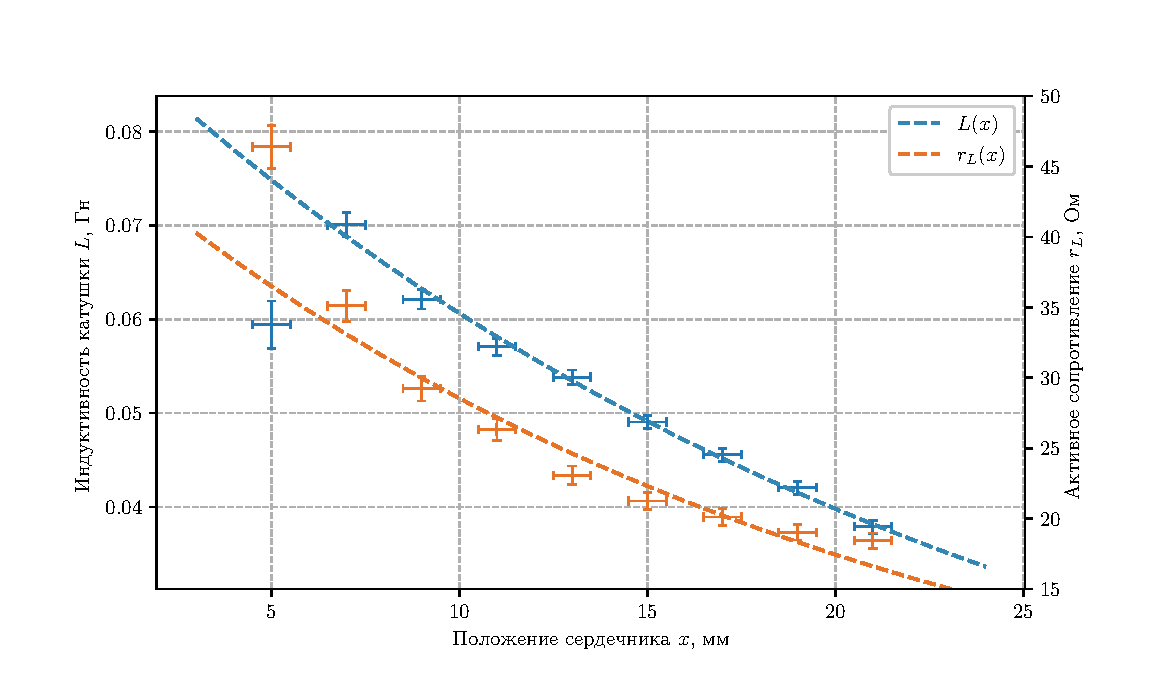
\includegraphics[width=\linewidth]{pics/LrL.eps}
	\caption{Зависимость $r_L$ и $L$ от $x$}
\end{figure}

Обратим внимание, что первые точки выпадают из основной серии, поэтому при аппроксимровании и расчетах не учитывались.

\begin{wrapfigure}{r}{0.4\textwidth}
    \centering
    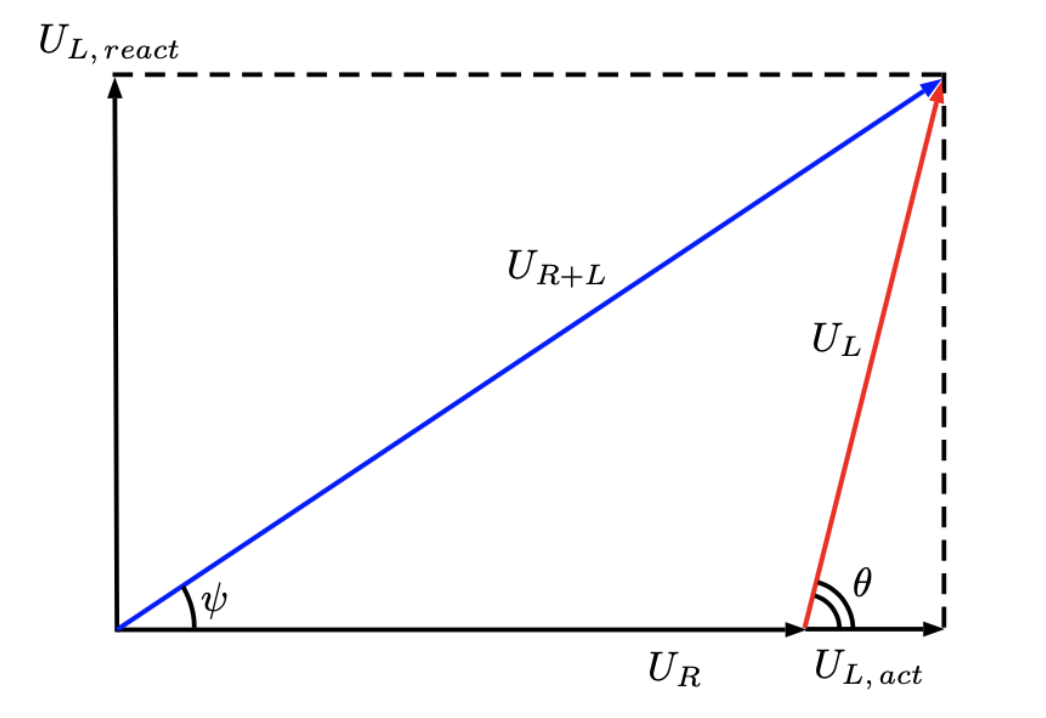
\includegraphics[width=\linewidth]{pics/vec.png}
    \caption{Векторная диаграмма}
\end{wrapfigure}

\subparagraph*{Векторная диаграмма.} 
Из векторной диаграммы (рис. 4) для среднего положения сердечника определим напряжение на активной $U_{L, акт}$ и реактивной $U_{L, реакт}$ части импеданса катушки.

\[\cos \psi = {U_R^2 + U_{LR}^2 - U_L^2 \over 2 U_RU_{LR}}\]

\[U_{L, акт} = U_{LR} \cos \psi - U_R,\quad U_{L, реакт} = U_{RL}\sqrt{1 - \cos^2 \psi}\]

Тогда $\cos \psi = 0.93 \pm 0.36$,

$ U_{L, акт} = 6.89 \pm 2.33\ В,\ U_{L, реакт} = 39.4 \pm 13.1\ В$
Теперь найдем $L$ и $r_L$:

$L = \dfrac{U_{L, реакт}}{I\Omega} = 0.13 \pm 0.05\ Гн,\ r_L = \dfrac{U_{L,акт}}{I} = 3.63 \pm 1.72\ Ом$

Определим по диаграмме $\cos \theta = \dfrac{U_{L, акт}}{U_L} = 0.11 \pm 0.05$
Экспериментальное значение $\cos \theta_{эксп} = \dfrac{P_L}{U_L I} = 0.33 \pm 0.02$, что довольно сильно разнится со знаением, полученным по векторной диаграмме.

Также по векторной диаграмме найдем $P_L = U_L I \cos \theta = 13.1 \pm 6.2$ Вт.
Из эксперимента $P_L = 38.0 \pm 0.5 Вт$, что также противоречит расчитанным значениям.

\subparagraph*{Добротность.}
Теперь расчитаем индуктивность и и сопротивление через добротность по формулам (6), (7), (8).
Элеткроемкость, при которой достигался резонанс равна $C = 52.1 \pm 1.1$ мкФ, $U_\Sigma = 65.5\pm 0.1$ В
\[L = {1 \over \omega_0 ^2 C} = 0.19 \pm 0.01\ Гн,\ r_L = {U_\Sigma\omega_0L \over C} = 75.2\pm 3\ Ом.\]

\subsection*{Подведение итогов}
Мы экспериментально исследовали резонанс напряжения в последовательной цепи переменного тока, а также нашли $ L $ и $ r_L $ различными методами. 
Вычисление $ r_L $ из векторной диаграммы имеет огромную погрешность. 
Это происходит из-за применения теоремы косинусов, применение которой вносит значительный вклад в погрешность, поскольку при её применении необходимо производить арифметические операции над числами, достаточно близко лежащими друг к другу. 
При этом их погрешность такова, что она не позволяет адекватно оценить значение искомой величины.

Остальные методы измерения сопротивления и индуктивности имеют право на существование, хотя и могут довольно сильно отличаться друг от друга. 

Таким образом, применённые методы позволяют оценить параметры катушки по порядку величины, однако они не дают возможности с точностью получить реальные характеристики элемента.

\end{document}